\chapter{Marco Teórico}
\label{chap:marco_teorico}

En este capítulo se presenta el marco teórico que sustenta el desarrollo de la aplicación web para la gestión centralizada de múltiples \textit{marketplaces}. Se abordan conceptos clave relacionados con el comercio en línea, sus dificultades y sus múltiples vertientes. Además, se exploran las tecnologías y herramientas utilizadas en el desarrollo de la aplicación, así como las metodologías de trabajo adoptadas durante el proceso.

\section{Comercio electrónico y canales de venta en línea}
\label{sec:comercio_canales}

En los últimos años, el comercio electrónico se ha convertido en una parte fundamental de la economía global. La capacidad de comprar y vender productos y servicios a través de internet ha transformado la forma en que las empresas interactúan con sus clientes. Este fenómeno ha dado lugar a la aparición de nuevos canales de venta, los llamados canales de venta en línea, que permiten a las empresas llegar a un público más amplio y diversificado, donde antes dependían de tiendas físicas o distribuidores locales.

No obstante, el comercio electrónico no es tan fácil como puede parecer en primera instancia. Existen tres grandes desafíos que las empresas deben enfrentar: la competencia, la infraestructura tecnológica y logística.

En internet todo el mundo juega con las mismas reglas; las facilidades que ofrece este medio son iguales para todos. El factor de proximidad al cliente ya no es el diferencial, sino la capacidad de ofrecer un producto o servicio que se diferencie del resto, tanto en calidad, precio o experiencia de compra. Esto genera que la competencia sea feroz, y las empresas deben encontrar formas innovadoras de destacar entre la multitud, tal como podrían ser las promociones, el marketing digital o la experiencia de usuario.

Por otro lado, el comercio electrónico requiere de una infraestructura tecnológica que permita listar productos, gestionar pedidos y pagos, y mantener una comunicación fluida con los clientes. Esto implica no solo contar con un sitio web atractivo y funcional, sino también con sistemas de gestión de inventario, plataformas de pago seguras y herramientas de análisis de datos que permitan tomar decisiones informadas. Todo esto puede resultar costoso y complicado de implementar, especialmente para pequeñas y medianas empresas que no cuentan con los recursos necesarios, ni en términos de personal, ni de dinero.

Por último, la logística es otro de los grandes retos del comercio electrónico. En el comercio tradicional, los productos se entregan directamente al cliente en la tienda. En el comercio electrónico, las empresas deben gestionar el almacenamiento, el envío y la entrega de productos a los clientes, lo que puede resultar complicado y costoso. La gestión de inventarios, la selección de proveedores de transporte y la coordinación de envíos son solo algunos de los aspectos logísticos que las empresas deben tener en cuenta para garantizar una experiencia de compra satisfactoria que cumpla con las expectativas de los clientes.

Estos tres factores son solo algunos de los muchos desafíos que enfrentan las empresas en el comercio electrónico. Por este mismo motivo, diferentes soluciones han surgido para ayudar a las empresas a superar estos obstáculos y aprovechar al máximo las oportunidades que ofrece el comercio en línea. Entre estas soluciones se encuentran dos que destacan por encima de las demás: las plataformas \textit{e-commerce} y los \textit{marketplaces}. Ambas ofrecen a las empresas la posibilidad de vender sus productos y servicios en línea, pero lo hacen de maneras diferentes.

\subsection{Plataformas \textit{E-commerce}}

Diseñar y programar una tienda en línea desde cero puede ser un proceso largo y costoso. Una tienda en línea no es una simple página web, sino un sistema complejo que debe gestionar una gran cantidad de información, como productos, precios, inventarios, pedidos y clientes.

Muchas empresas optan por utilizar las llamadas plataformas \textit{e-commerce}. Una plataforma \textit{e-commerce} es una aplicación que permite a las empresas crear y gestionar su propia tienda en línea en relativamente pocos pasos. Existen muchas plataformas \textit{e-commerce}, pero todas se caracterizan por ofrecer una serie de herramientas y funcionalidades por defecto de manera que las empresas puedan crear su tienda en línea sin necesidad de tener conocimientos técnicos avanzados. Estas plataformas suelen incluir plantillas de diseño, sistemas de gestión de inventario, herramientas de marketing y análisis, y opciones de pago seguras. Además, muchas de ellas ofrecen integraciones con otros servicios y funcionalidades adicionales, todo bajo los llamados \textit{plugins} \cite{adobe_ecommerce_platforms}.

Todo este conjunto de facilidades hacen que el uso de plataformas \textit{e-commerce} sea una opción atractiva para muchas empresas, especialmente para aquellas que están comenzando en el comercio electrónico o que no cuentan con los recursos necesarios para desarrollar su propia tienda en línea desde cero. Sin embargo, también existen desventajas asociadas al uso de estas plataformas. Por ejemplo, las empresas pueden tener menos control sobre el diseño y la funcionalidad de su tienda en línea, y pueden estar sujetas a las políticas y tarifas de la plataforma, entre muchas otras cosas. Además, algunas plataformas pueden no ser escalables o flexibles lo suficiente como para adaptarse a las necesidades cambiantes de una empresa en crecimiento.

Existe una amplia variedad de plataformas \textit{e-commerce} en el mercado, cada una con sus propias características y funcionalidades. Algunas de las más populares son Shopify, WooCommerce (\textit{plugin} de WordPress), Magento y PrestaShop. Cada una de estas plataformas tiene sus propias ventajas y desventajas, y la elección de la plataforma adecuada dependerá de las necesidades, objetivos específicos y las dimensiones de cada empresa.

\subsection{\textit{Marketplaces}}

Los \textit{marketplaces} son plataformas en línea que permiten a las empresas vender sus productos y servicios a través de un canal de venta compartido. A diferencia de las plataformas \textit{e-commerce}, donde las empresas crean y gestionan su propia tienda en línea, los \textit{marketplaces} permiten a las empresas listar sus productos y servicios junto con los de otras empresas en una única plataforma. Esto significa que las empresas pueden aprovechar la audiencia y el tráfico del \textit{marketplace} para llegar a nuevos clientes sin necesidad de invertir en marketing o publicidad.

Aquí radica realmente la ventaja de los \textit{marketplaces}: la posibilidad de llegar a un público más amplio y diversificado sin necesidad de invertir grandes cantidades de dinero en marketing o publicidad. Tanto en los \textit{e-commerce} tradicionales (tiendas en línea creadas desde cero) como en las plataformas \textit{e-commerce}, las empresas deben invertir considerables cantidades de dinero para atraer tráfico a su tienda en línea, mientras que en los \textit{marketplaces} el tráfico ya está allí, lo que significa que las empresas pueden aprovecharlo para aumentar sus ventas y llegar a nuevos clientes.

No obstante, este tipo de plataformas también tienen sus desventajas. En primer lugar, todos los productos acostumbran a estar bajo una comisión de manera que la empresa o bien debe subir el precio de su producto o asumir la pérdida de margen. Está comisión puede rondar entre el 10\% y el 20\%. En segundo lugar, los \textit{marketplaces} pueden ser muy competitivos, pues un mismo producto puede ser vendido por distintas empresas, dando lugar a una guerra de precios que puede afectar la rentabilidad de las empresas. Por último, en un \textit{marketplace} la empresa no tiene ningún tipo de control sobre la experiencia de compra del cliente, lo que puede afectar la percepción de la marca y la lealtad del cliente, además de que debe someterse a la política de la plataforma, que muchas veces puede no ser beneficiosa para la empresa y puede llegar a afectar sus operaciones.

Existen múltiples \textit{marketplaces}, tanto de productos físicos, como Amazon, eBay o AliExpress, como de productos digitales o servicios, como Udemy, Uber o Glovo. Cada uno de estos tiene sus propias características y funcionalidades, y la elección del \textit{marketplace} adecuado dependerá de las necesidades y objetivos específicos de cada empresa. Es importante destacar que el uso de una plataforma \textit{e-commerce} no excluye la posibilidad de listar productos o servicios en un \textit{marketplace}. De hecho, muchas empresas optan por combinar ambas estrategias para maximizar su alcance y diversificar sus canales de venta, aprovechando las ventajas que ofrece cada una de estas opciones \cite{sharetribe_marketplac_platforms}.

% \section{Modelos de distribución de software SaaS}
\label{sec:modelos_negocio}

Hay una gran variedad de modelos de distribución de software, tal como pueden ser el modelo \textit{On-Premise}, el modelo \textit{Infrastructure as a Service} (IaaS) o el modelo \textit{Platform as a Service} (PaaS). Sin embargo, el modelo que más se utiliza en la actualidad es el modelo \textit{Software as a Service} (SaaS).

Años atrás, el software se distribuía principalmente a través de licencias perpetuas, donde los usuarios compraban una licencia para utilizar el software en sus propios servidores o computadoras. Este modelo requería que los usuarios gestionaran la infraestructura y el mantenimiento del software, lo que podía ser costoso y complicado. Esto significaba que el proveedor del software simplemente facilitaba el producto y el usuario debía hacerse cargo de la instalación, configuración y mantenimiento del mismo. Esto podía resultar complicado y costoso, especialmente para pequeñas y medianas empresas que no contaban con los recursos necesarios para gestionar su propia infraestructura. Esto es conocido como una infraestructura \textit{On-Premise}.

Con la llegada de internet y la nube, surgieron nuevos modelos de distribución de software que permitieron a las empresas ofrecer sus productos y servicios de manera más eficiente y escalable. El modelo SaaS es uno de los más populares y se basa en la idea de que el software se aloja en la nube y se accede a través de internet. Esto significa que los usuarios no necesitan instalar ni gestionar el software en sus propios servidores u ordenadores, sino que pueden acceder a él a través de un navegador web.

Sin embargo, la dependencia de la conexión a internet, la falta de control sobre la infraestructura y la seguridad de los datos son puntos críticos en el modelo. Además, los proveedores de SaaS suelen cobrar tarifas mensuales o anuales por el uso del software, pues el mantenimiento de la infraestructura y el soporte técnico son responsabilidad del proveedor.

Existen también otras alternativas, como pueden ser los modelos IaaS y PaaS. Cada uno de estos modelos tiene sus propias ventajas y desventajas, y dependiendo del tipo de negocio y las necesidades del cliente, uno puede ser más adecuado que otro. En la figura \ref{fig:modelos_negocio} se pueden observar los diferentes modelos de distribución de software y sus características.

\begin{figure}
    \centering
    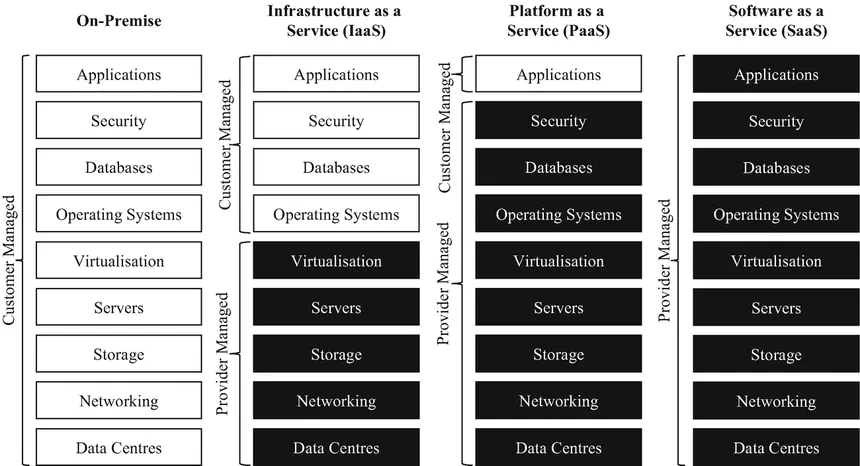
\includegraphics[width=0.8\textwidth]{figures/theoric_frame/comp_services.png}
    \caption{Modelos de distribución de software. Fuente: \cite{modelos_distirbucion}}
    \label{fig:modelos_negocio}
\end{figure}

\section{Arquitectura y tecnologías de una aplicación web}
\label{sec:arquitectura_sistema}

En el mundo del software existen dos tipos de aplicaciones: las aplicaciones de escritorio y las aplicaciones web. Las aplicaciones de escritorio son aquellas que se instalan en un ordenador y se ejecutan de forma local, mientras que las aplicaciones web son aquellas que se ejecutan en un servidor y se acceden a través de un navegador web.

Desde los inicios del desarrollo de software, las aplicaciones de escritorio han sido la norma. Sin embargo, en los últimos años ha habido un cambio significativo hacia el desarrollo de aplicaciones web, pues el avance de las distintas tecnologías web y la conectividad a internet han mitigado considerablemente las desventajas que anteriormente presentaban.

BENEFICIOS Y DESVENTAJAS APLICACIONES DE escritorio

BENEFICIOS Y DESVENTAJAS APLICACIONES WEB

\subsection{Arquitecturas web}

\subsection{Tecnologías web}